\subsection{Carnot Cycle}\label{subsec:Carnot_Cycle}
The \nameref{def:Process} path of the \nameref{def:Carnot_Cycle} is shown in \Cref{fig:Carnot_Cycle}.

\begin{figure}[h!tbp]
  \centering
  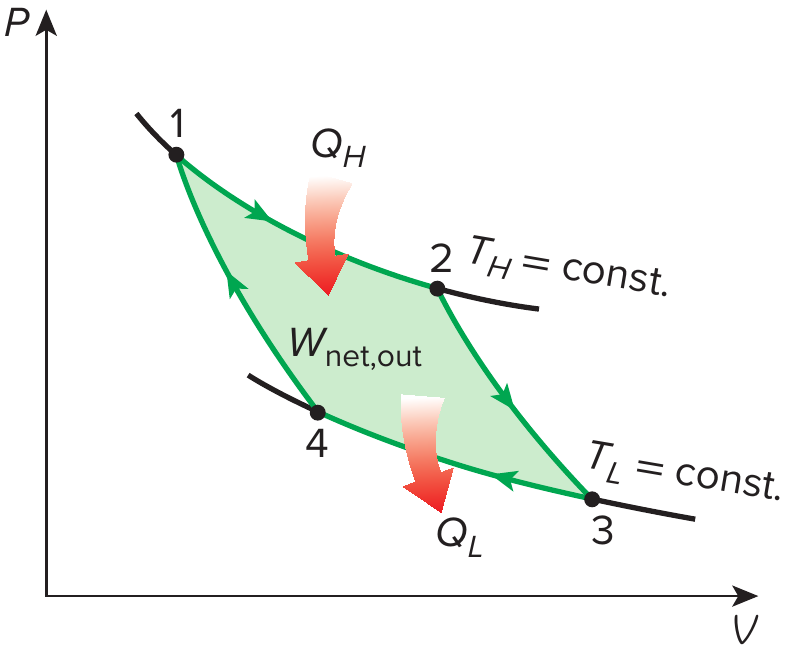
\includegraphics[scale=0.75]{Carnot_Cycle.png}
  \caption{Carnot Cycle (\cite[pg. 252]{ThermoTextbook})}
  \label{fig:Carnot_Cycle}
\end{figure}

\begin{definition}[Carnot Cycle]\label{def:Carnot_Cycle}
  The \emph{Carnot cycle} is a thermodynamically ideal \nameref{def:Cycle}.
  The temperatures $\Temp_{H}$ and $\Temp_{L}$ are isotherms.
  The vertical cases are times when the \nameref{def:System} is perfectly \nameref{def:Adiabatic}, meaning only \nameref{def:Work}, $\Work$, is done.
  The interior of the cycle's process path is the net work done by the \nameref{def:System}.
\end{definition}

If we look at the efficiency of the \nameref{def:Carnot_Cycle}, we see something interesting.
\begin{align*}
  \Efficiency_{C} &= 1 - \frac{\Heat_{Out}}{\Heat_{In}} \\
                  &= 1 - \frac{\Heat_{Out} \propto \Temp_{L}}{\Heat_{In} \propto \Temp_{H}} \\
                  &= 1 - \frac{\Temp_{L}}{\Temp_{H}}
\end{align*}


%%% Local Variables:
%%% mode: latex
%%% TeX-master: "../../MMAE_320-Thermo-Reference_Sheet"
%%% End:
